\section{Methodology}

Given a dataset $D$ with $n$ variables, $m$ of which are considered sensitive or protected and one label in a classification task, the objective of equalized odds is to learn a model which performs equally well (be it any of accuracy, AUROC, false positive rate, true positive rate, etc) on each of the subgroups. With a complementary objective of achieving the highest overall performance, we would expect to achieve a trade-off between the two with some subgroups benefiting in performance at the cost of degradation for the others. However, in a true toy joint data distribution for two binary sensitive variables $A$ and $B$, a confounding variable $C$ and the target label $T_0$, \\
\begin{center}
Let A, B be Bernoulli random variables :
\[A \sim Bern(p)\]
\[B \sim Bern(p)\]

where $p=.5$
\begin{equation}
    Bern(p) = f(k;p) =
    \left\{
        \begin{array}{cc}
                p & \mathrm{if\ } k=1 \\
                1-p & \mathrm{if\ } k=0 \\
        \end{array} 
    \right.
\end{equation}
with a selected constant $0<c<p$
\[ C = 
\begin{cases}
\mathcal{U}(0,1) & if B = 0\\
\mathcal{N}(p, \sigma^2) - c & if B = 1, A= 0\\
\mathcal{N}(p, \sigma^2) + c & if B = 1, A= 1 \\
\end{cases}
\]

$T_0 \sim Bern(C)$ \\
\end{center}
In this scenario, there are two subgroups for which $B=0$, the confounding variable $C$ has uniform random values and for the two subgroups which have $B=1$, the confounding variable $C$ is distributed normally with means at two different values separated by a constant. Suppose we were to train a bias mitigation model $M$, which uses only the perceived non-sensitive variable "C" as the feature to classify to identify target label $T_0$  in order to achieve equal performance in terms of accuracy. While trying to increase overall accuracy, there is a potential trade-off where the algorithm could penalize two subgroups identified by $B=1$, without any gain in the subgroups identified by $B=0$. Effectively, this implies that two subgroups are penalized to ensure that accuracy is close to the uniformly random accuracy as in the other two subgroups as shown in Figure \ref{pareto}. This is counter-productive for each of the subgroup's performance in question. Hence, it is necessary to guard against such scenarios, by explicitly accounting for this edge-case.

\begin{figure}[htbp]
	\begin{center}
		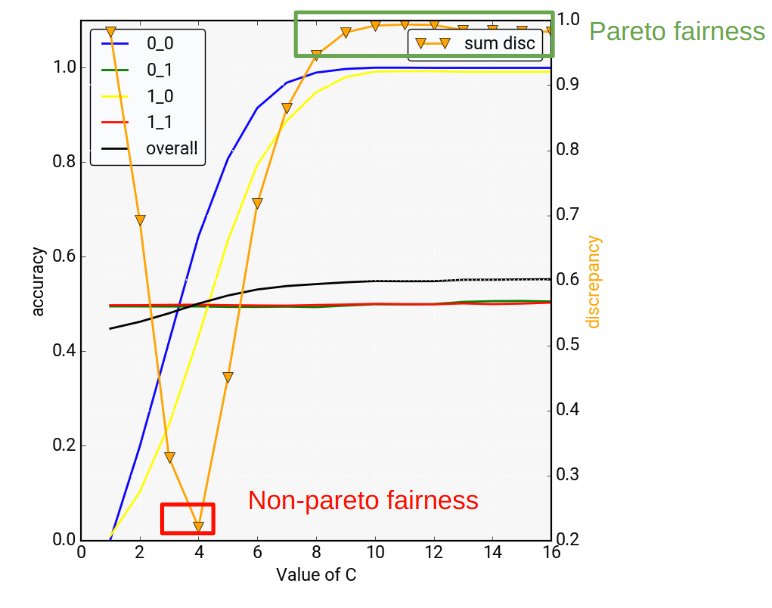
\includegraphics[width=3.2in,height=2in]{pareto.png} 
        \setlength{\belowcaptionskip}{-8pt} 
		\caption{Synthetic dataset where Pareto Efficient fairness is desirable}
		\label{pareto}
	\end{center}
\end{figure}

Our proposal is inspired from the hypothesis that the optimization should aim for "potentially optimal" performance for each of the subgroups and that "optimal" performance can be calibrated differently for different subgroups. This is similar to current research which highlights the benefits of transparency over fairness, where it is acceptable to understand the differences between various subgroups' performance in the dataset and operate in a way to correct them as opposed to fairness through blindness. Since each subgroup tries to achieve its own "optimal" performance during the course of the bias mitigation, this can be thought of achieving Pareto-efficiency, where we try to optimize for overall performance, while accepting decrease in performance for certain subgroups if and only if there is at least one subgroup which benefits as a result. We also want to ensure that the penalty is not dominated by only certain subgroups, but shared across subgroups equitably. These two constraints can be thought of as constraining the initial performance optimization objective while
minimizing the full Pareto loss $L_{p}(o, \hat{o})$. The bias mitigation objective can be specified as

\[ L_{b}(o, \hat{o}) =\min \sum{P(g)} \]
where 
\[ P(g) = Relu(F_{opt}[g] - F[g]) \]

and
$P(g \in G) < \epsilon$ for all subgroups $g$,
where G is the power set containing all possible subgroups over the set of sensitive variables $S$, $F_{opt}[g]$ is the heuristic optimal evaluation score for subgroup $g$ and $F[g]$ is the actual evaluation score for a given model and Relu is a linear activation function to avoid penalizing scores that achieve results better than the heuristic optimal one.

These constraints were relaxed through Lagrangian dual formulation similar to \cite{Eban2016} with the appropriate loss weight ($\lambda$), along with a cross entropy classification loss: $L_{ce}(o, \hat{o})$ to yield

\[ L_{p}(o, \hat{o}) = \sum(L_{ce}(o, \hat{o})) + \lambda( \sum{P(g)} + |P(g) - \epsilon| ) \]

\subsubsection{Multiple metrics of fairness}
One of the drawbacks of existing approaches, is that it isn't applied to multiple metrics of fairness like false positive rate and false negative rates simultaneously. However, the above Pareto loss can be scaled easily to mitigate discrepancy for many metrics. We achieve this by defining a penalty term per metric of fairness, weighted by separate lambdas signifying the trade-offs between the multiple Lagrangian relaxation terms. In our evaluation, we do this with an equal weighting between FPR and FNR to overcome the drawbacks of metrics like accuracy which obfuscate the type of errors in a model.

\subsection{Confounding variable detection and interpretation of fairness}
During the exploration of subgroup fairness, we were also faced with the challenge of identifying which variables were sensitive and which were not. This is usually done by the domain expert and is known ahead of time. However, due to confounding causal variables, it could be that some of the features used are highly correlated with the sensitive variable in question. It has been shown in Kilbertus et al [3] that arguing about fairness purely based on observational data is not feasible and hence the domain experts have to make decisions whether or not a particular confounding variable's bias is to be permitted. We now propose a process through which these domain experts can be aided by being presented the potential confounding variables for their decision. We present our approach based on quantifying the discrepancy in subgroup fairness in Algorithm \ref{alg:algorithm-confound} to identify potential resolving confounding variables through which we can explain the seeming bias.
 
\begin{algorithm}
\caption{Outline of Procedure for Potential Confounding Variable Detection}
\label{alg:algorithm-confound}
Given a set of sensitive features $S$, and the remaining features $F$ and a model $M$ which is  a binary classifier using the full set of features, if it turns out that the performance of $M$ on groups defined by membership in $S$ have discrepancy, we perform the following test before qualifying a model unfair.\\
For each feature $f$ in $F$, we split the population into groups based on $f$ first, and then split into subgroups based on $G$, the power set of $S$, within each of the groups.\\
We then evaluate the model $M$ on each of the subgroups and compare the performance across the subgroups.\\
For each subgroup $g \in G$, we quantify the sum of discrepancies between subgroup performance as $d[f, g]$.\\
We also quantify the lack of samples in each of the subgroups by calculating the confidence intervals of the discrepancies.\\
In some cases, some subgroups don't have enough samples to even calculate discrepancy. This is quite dangerous to ignore as we might be hiding a potentially sensitive variable whose distribution matches with one of the sensitive variables.\\
This kind of sample insufficiency will be quantified by the proportion of the population which was ignored in Step 5.\\
The confounding variable will minimize the discrepancy in Step 4, while maintaining that enough proportion of the population was used in the calculation (Step 5).\\
These are two trade-offs which can be modeled by the domain expert.\\
Return the confounding variable which can be argued as a reasoning for fairness if the discrepancy calculated in Step 4 is close to zero.\\
\end{algorithm}

We will argue the other case (where it seems fair, but could be interpreted given further information as not) similarly. Only, in that case, we aim to identify variables which maximize discrepancy instead of minimizing. Since these variables expose subgroup bias when conditioned on them, these can also be considered potentially sensitive if the domain expert determines that the bias from such confounding variables are to be mitigated. We present the next few sections assuming that the set of sensitive variables are already updated with some of these confounding variables included as determined by the domain expert.

\subsection{Pareto-Efficent Algorithm}
In order to obtain a heuristic of the optimal subgroup performance, we use the performance achieved when trained purely on the subgroup's data in question. We understand that this isn't the best estimate in many cases, especially where prevalence of subgroups are varied, and majority subgroups benefit from a large dataset, whereas minority subgroups can be penalized as we avoid any transfer learning \cite{PapernotAEGT16}. We hence propose an iterative approach where this heuristic would be updated in each iteration if the optimal subgroup performance was bettered by a jointly trained model. In the rest of the evaluation, we present results from the heuristic initialized with the separately trained performance for better understanding of our approach. Once we obtain the heuristic optimal performances, we input them into the jointly training Pareto bias mitigation algorithm, which minimizes the loss $L_p$ mentioned above for every batch. We further ensure that the batch used at every loss minimization is representative of the subgroup distribution present in the original dataset.

\begin{algorithm}
\caption{Iterative Pareto-Efficient Bias Mitigation}
\label{alg:algorithm-pareto}
\begin{algorithmic}
\STATE{G = $\mathcal{P}(S)$ where S is the membership set of sensitive variables}
\STATE{$F_{opt}(g) = eval(M_{g}, D_{g})$  $\forall g \in G$, $M_{g}$ is the model trained and evaluated on only $D_{g}$, data with subgroup g}
\STATE{$F = \{\}$}
\WHILE{F is $\{\}$ or $\exists g, F[g] > F_{opt}[g]$}
\STATE{Update $F_{opt}[g] = F[g]$ if $F[g] > F_{opt}[g]$}
\STATE{Train M to minimize $L_p$ for the updated $F_{opt}$}
\STATE{$F[g] = eval(M, D_{g})$}
\ENDWHILE
\end{algorithmic}
\end{algorithm}

\subsection{Bias Loss Weights}
The loss to be minimized contains a single bias loss weight term which we use to control the trade off between overall accuracy and achieving Pareto-efficient levels for each of the subgroups with equal penalty per subgroup. This term influences the decisions and changing this weight further exemplifies the difference between the equalized odds loss and the Pareto loss as can be seen in Figure \ref{bias_weight}. As we increase the bias weight, we see that the Pareto loss bias mitigation moves to other Pareto-efficient levels with higher overall accuracy, whereas the equalized loss moves towards the undesired operating point where discrepancy across subgroups is minimized regardless of improvement in accuracy by at least one of the subgroups. We can also weigh the discrepancies of each of the subgroups differently, but our synthetic datasets did not warrant it. We leave it to the practitioner to correspondingly set these weights per subgroup or as a constant as needed. 

\begin{figure*}[htbp]
	\begin{center}
		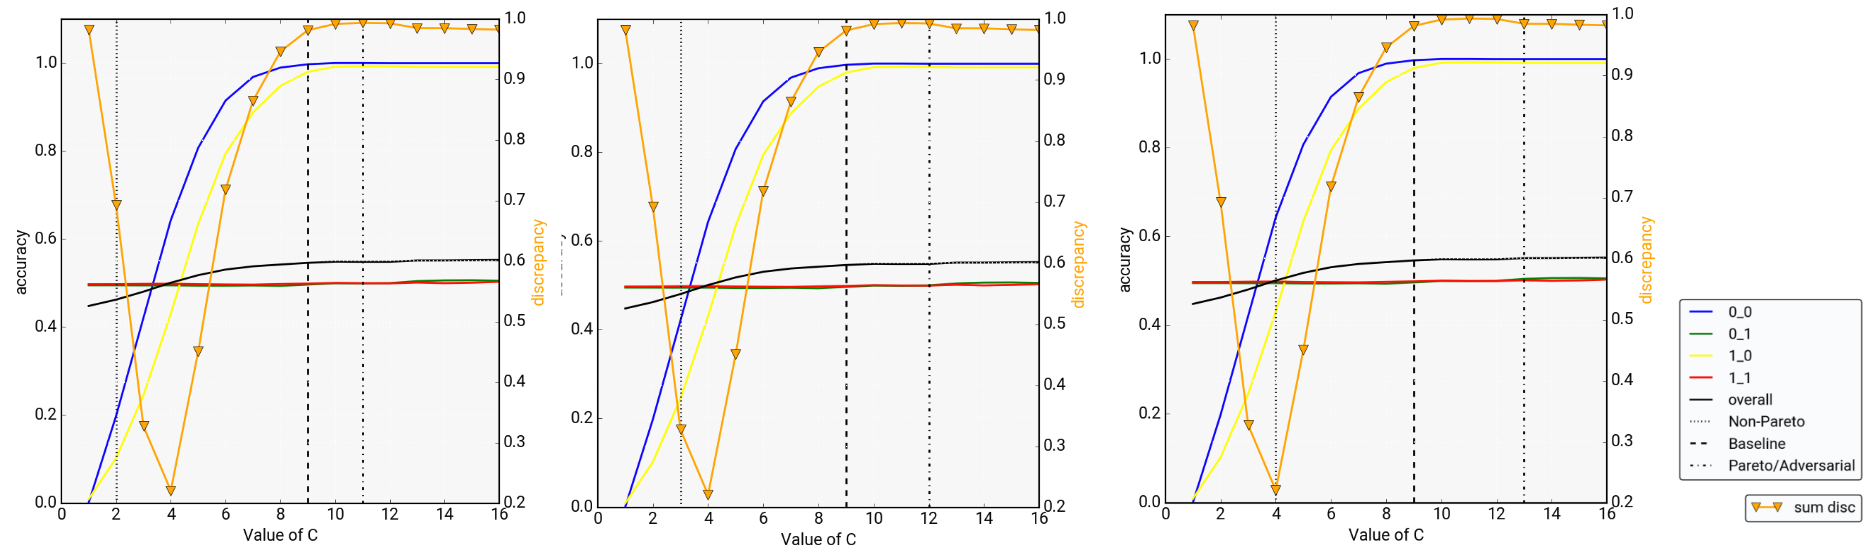
\includegraphics[width=7.5in,height=2.4in]{bias_weight.png} 
        \setlength{\belowcaptionskip}{-8pt} 
		\caption{Effect of bias weight on bias trade-offs}
		\label{bias_weight}
	\end{center}
\end{figure*}

\subsection{Prevalence}
Prevalence usually varies between subgroups and some minority subgroups could be ignored during bias mitigation. The appproach mentioned in Kearns et al. \cite{Kearns2017PreventingFG} defines discrepancies factoring the population ratio of each of the subgroups. This can have perverse effects on these subgroups as their performance deviating from either the overall performance or the Pareto-efficient level can be ignored while optimizing the loss function. This is clearly seen in Figure \ref{prevalence} where the discrepancy curve representing the discrepancy from the overall performance can be seen to have lowered and smoothened when multiplied with the subgroup's population ratio. This can be quite deceiving where the majority subgroup, which also guides the overall performance dominates the sum of discrepancy loss too. Hence, we guard against such prevalence based weighting.

\begin{figure}[htbp]
	\begin{center}
		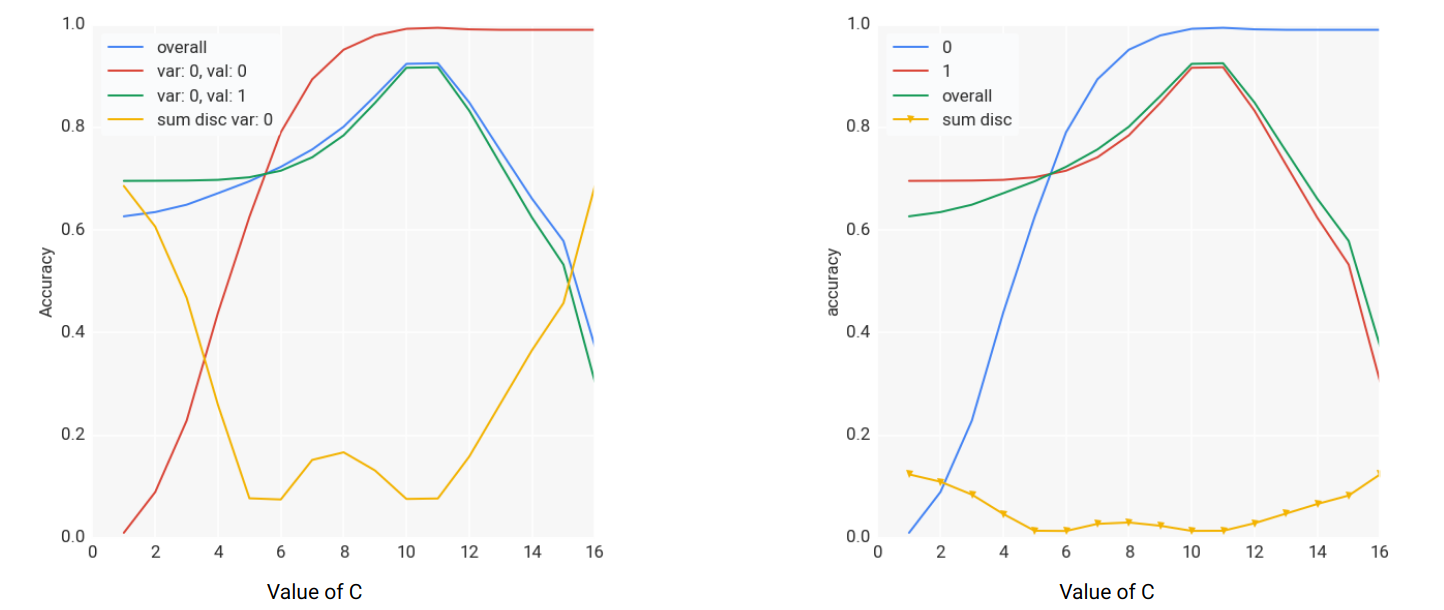
\includegraphics[width=3.2in,height=2.0in]{prevalence.png} 
        \setlength{\belowcaptionskip}{-8pt} 
		\caption{Weighing discrepancy by prevalence ignores the minority subgroup}
		\label{prevalence}
	\end{center}
\end{figure}




 
 


